\section{Evaluation}
\label{sec:evaluation}

We evaluate EVICT through four measured studies and one explicitly projected frontier-model outlook. Every table reports the study setting in its caption because repeated model names appear under different sample sets and methods.

\subsection{RQ1: How Do Lite LLMs Perform Zero-Shot?}

Study~1 evaluates five lite LLMs on Juliet alerts spanning 87+ CWE classes with the base schema prompt, $k_{\mathrm{sc}}=1$, and no conformal calibration. Coverage is the pre-escalation accepted-decision rate.

\begin{table}[t]
\centering
\caption{Study~1 zero-shot baseline on Juliet (87+ CWE classes, $k_{\mathrm{sc}}=1$, no conformal calibration). All metrics are pre-escalation.}
\label{tab:multimodel}
\small
\setlength{\tabcolsep}{4pt}
\resizebox{\linewidth}{!}{%
\begin{tabular}{lrrrrrr}
\toprule
\textbf{Model} & \textbf{Alerts} & \textbf{Coverage (pre-escal.)} & \textbf{Precision (pre-escal.)} & \textbf{Recall (pre-escal.)} & \textbf{FP Mitig. (pre-escal.)} & \textbf{ECE (pre-escal.)} \\
\midrule
Claude Haiku 4.5 & 3,061 & 97.5\% & \textbf{59.9\%} & 36.8\% & \textbf{80.3\%} & \textbf{0.358} \\
Gemini 3.1 Flash Lite Preview & 991 & 56.0\% & 48.0\% & 37.4\% & 24.4\% & 0.465 \\
Gemini 2.5 Flash Lite & 2,663 & 82.8\% & 46.8\% & 64.4\% & 26.5\% & 0.483 \\
GPT-5 Nano & 1,045 & 98.0\% & 44.9\% & 78.1\% & 17.9\% & 0.538 \\
GPT-4o Mini & 3,107 & \textbf{98.8\%} & 42.2\% & \textbf{90.8\%} & 13.0\% & 0.547 \\
\bottomrule
\end{tabular}}
\end{table}

Zero-shot lite models are not deployment-ready triagers. In Study~1, precision spans 42.2--59.9\% and every ECE exceeds 0.35. The models also split into operational profiles: Claude Haiku 4.5 is conservative (59.9\% precision, 36.8\% recall, 80.3\% FP mitigation), while GPT-4o Mini is aggressive (90.8\% recall, 13.0\% FP mitigation). This motivates selective prediction: different models trade off missed vulnerabilities and developer burden, but none provides calibrated reliability out of the box.

\subsection{RQ2: What Determines Calibration Effectiveness?}

Study~2 is the central conformal experiment: 247 Juliet alerts from CWE-89/78/190, $k_{\mathrm{sc}}=5$, $F=5$ cross-validation folds, and target conformal miscoverage $\alpha_{\mathrm{conf}}=0.1$. It spans six models and three training paradigms.

\begin{table}[t]
\centering
\caption{Study~2 multi-model conformal calibration on 247 Juliet alerts (CWE-89/78/190, $k_{\mathrm{sc}}=5$, $F=5$, $\alpha_{\mathrm{conf}}=0.1$). Metrics are pre-escalation singleton-reject results.}
\label{tab:conformal_multimodel}
\small
\setlength{\tabcolsep}{3.5pt}
\resizebox{\linewidth}{!}{%
\begin{tabular}{llcccccc}
\toprule
\textbf{Model} & \textbf{Type} & \textbf{Precision (pre-escal.)} & \textbf{Recall (pre-escal.)} & \textbf{ECE (pre-escal.)} & \textbf{Coverage (pre-escal.)} & \textbf{Unanimous} & \textbf{Calib. $\Delta$P} \\
\midrule
\textbf{R1-Distill-14B} & 14B RL-reasoning & \textbf{40.0\%} & 71.9\% & \textbf{0.335} & 98.4\% & \textbf{36\%} & +1.1pp \\
Claude Haiku 4.5 & Frontier lite & \textbf{47.4\%} & 34.5\% & 0.373 & 95.9\% & 90\% & +1.7pp \\
GLM-4-9B-Chat & 9B instruct & 38.0\% & 95.9\% & 0.513 & 96.3\% & 61\% & +1.1pp \\
Gemini 2.5 Flash Lite & Lite instruct & 38.9\% & 95.5\% & 0.555 & 97.6\% & 85\% & $<$1pp \\
DS-Coder-V2-Lite & 16B MoE code & 37.6\% & 100\% & 0.620 & 98.0\% & 98\% & $<$1pp \\
Qwen-Coder-32B & 32B code & 37.0\% & 81.5\% & 0.565 & 98.0\% & 86\% & $<$1pp \\
\bottomrule
\end{tabular}}
\end{table}

Study~2 shows that confidence quality, not model size, limits conformal calibration in this setting. R1-Distill-14B produces 36\% unanimous votes and ECE 0.335, while instruction-tuned and code-specialized models produce 85--98\% unanimity and ECE 0.51--0.62. The six-model sample is too small for a statistical claim about training objective as a population property, but the 49--62pp unanimity gap between R1-Distill-14B and the standard/code models is a large effect consistent with a mechanistic explanation: reasoning traces create genuine sample disagreement when evidence is ambiguous.

Claude Haiku 4.5 illustrates a second path to acceptable calibration. In Study~2 it has 90\% unanimity, but its higher accepted-alert precision (47.4\%) yields ECE 0.373. Thus EVICT can obtain usable calibration either from diverse confidence or from high base precision; the ideal model combines both.

\begin{figure}[t]
\centering
\resizebox{0.88\linewidth}{!}{%
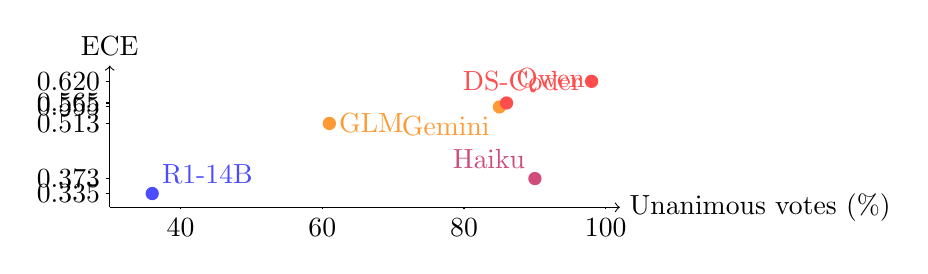
\begin{tikzpicture}[x=0.09cm,y=5.0cm]
\draw[->] (30,0.30) -- (102,0.30) node[right] {Unanimous votes (\%)};
\draw[->] (30,0.30) -- (30,0.66) node[above] {ECE};
\foreach \x in {40,60,80,100} \draw (\x,0.30) -- (\x,0.295) node[below] {\x};
\foreach \y/\lab in {0.335/0.335,0.373/0.373,0.513/0.513,0.555/0.555,0.565/0.565,0.620/0.620} \draw (29.5,\y) -- (30,\y) node[left] {\lab};
\fill[blue!70] (36,0.335) circle (2.4pt) node[above right] {R1-14B};
\fill[purple!70] (90,0.373) circle (2.4pt) node[above left] {Haiku};
\fill[orange!80] (61,0.513) circle (2.4pt) node[right] {GLM};
\fill[orange!80] (85,0.555) circle (2.4pt) node[below left] {Gemini};
\fill[red!70] (98,0.620) circle (2.4pt) node[left] {DS-Coder};
\fill[red!70] (86,0.565) circle (2.4pt) node[above right] {Qwen};
\end{tikzpicture}}
\Description{Scatter plot of Study 2 models with vote unanimity on the horizontal axis and ECE on the vertical axis. R1-Distill has low unanimity and low ECE, while code-specialized models cluster at high unanimity and high ECE.}
\caption{Study~2 confidence-signal map. The six-model pattern links high unanimity with poor ECE, except Claude Haiku 4.5, whose higher base precision offsets degenerate votes.}
\label{fig:confidence_signal}
\end{figure}

\subsection{RQ3: Does the Pipeline Transfer to Real Alerts?}

Study~3 evaluates 549 CodeQL alerts from 45 CWE-Bench-Java projects with $k_{\mathrm{sc}}=1$. Ground truth contains 17 TP and 532 FP, a 97\% FP base rate. These are pre-escalation LLM decisions without conformal cross-validation.

\begin{table}[t]
\centering
\caption{Study~3 real-world validation on 549 CWE-Bench-Java CodeQL alerts from 45 projects ($k_{\mathrm{sc}}=1$). Metrics are pre-escalation.}
\label{tab:cwebench}
\small
\setlength{\tabcolsep}{3.5pt}
\resizebox{\linewidth}{!}{%
\begin{tabular}{lccccccc}
\toprule
\textbf{Model} & \textbf{Precision (pre-escal.)} & \textbf{Recall (pre-escal.)} & \textbf{F1 (pre-escal.)} & \textbf{TN (pre-escal.)} & \textbf{ABSTAIN (pre-escal.)} & \textbf{Pred. TP} & \textbf{Pred. FP} \\
\midrule
DS-Coder-V2-Lite & \textbf{4.0\%} & 82.4\% & \textbf{0.080} & \textbf{184} & 10 (2\%) & 352 & 187 \\
Gemini 2.5 Flash Lite & 3.3\% & 93.3\% & 0.063 & 47 & 73 (13\%) & 428 & 48 \\
R1-Distill-14B & 3.0\% & \textbf{100\%} & 0.060 & 32 & 77 (14\%) & 440 & 32 \\
GLM-4-9B-Chat & 1.9\% & 62.5\% & 0.040 & 97 & 185 (34\%) & 264 & 100 \\
Qwen-Coder-32B & 1.5\% & 40.0\% & 0.030 & 76 & 340 (62\%) & 130 & 79 \\
\bottomrule
\end{tabular}}
\end{table}

Study~3 reveals the code-specialization paradox. DS-Coder-V2-Lite has the worst confidence quality in Study~2 (98\% unanimous, ECE 0.620) but the best real-world precision in Study~3 (4.0\%) and the highest true-negative count (184 vs. 32--97 for the other reported models). Code-specialized training appears to improve recognition of safe code patterns while worsening uncertainty quantification. A separate R1-Distill-14B $k_{\mathrm{sc}}=5$ sample of 100 CWE-Bench-Java alerts preserves diverse confidence: 46\% unanimous, confidence distribution \{0.4:1, 0.6:24, 0.8:29, 1.0:46\}, and 10\% abstention.

\subsection{RQ4: Can Prompt Design Substitute for Scale?}

Study~4 holds Gemini 2.5 Flash Lite fixed on the same 247-alert Juliet CWE-89/78/190 subset as Study~2 and changes only the prompt. The default prompt asks for evidence-conditioned classification. The contrastive prompt forces the model to build TP and FP arguments before deciding.

\begin{table}[t]
\centering
\caption{Study~4 prompt comparison on Gemini 2.5 Flash Lite (247 Juliet alerts, $k_{\mathrm{sc}}=5$). Metrics are pre-escalation singleton-reject results.}
\label{tab:prompt_strategy}
\small
\begin{tabular}{lcccccc}
\toprule
\textbf{Prompt} & \textbf{Unanimous} & \textbf{ECE (pre-escal.)} & \textbf{$\hat q$} & \textbf{Coverage (pre-escal.)} & \textbf{ABSTAIN (pre-escal.)} & \textbf{Precision (pre-escal.)} \\
\midrule
Default & 84.6\% & 0.555 & 0.20 & 97.6\% & 0\% & 38.9\% \\
\textbf{Contrastive} & \textbf{16.2\%} & \textbf{0.337} & \textbf{0.60} & 70.6\% & 29.1\% & 37.9\% \\
\bottomrule
\end{tabular}
\end{table}

The contrastive prompt is the paper's cleanest causal comparison because the model and alert set are fixed. It reduces ECE by 39\% and unanimity by 68.4pp. It also produces more diverse confidence than R1-Distill-14B under the default Study~2 prompt (16.2\% vs. 36\% unanimous). The trade-off is over-conservatism: coverage drops to 70.6\% and LLM-level abstention rises to 29.1\%. The result still changes the design space: cheap lite models can become calibratable if the prompt elicits genuine uncertainty.

\subsection{RQ5: Projected Outlook for Frontier Reasoning Models}
\label{sec:frontier_projections}

RQ5 is an extrapolation, not a measured empirical study. We project frontier-model behavior from the mechanistic model supported by Studies~2 and~4: conformal calibration is useful when a model combines high base precision with diverse confidence. Full multi-model frontier evaluation with $k_{\mathrm{sc}}=5$ and conformal cross-validation was outside this study's budget. We therefore release the benchmark harness and projection method so groups with the required API budget can run the test directly.

\begin{table}[t]
\centering
\caption{RQ5 projected frontier outlook. These are estimates, not measured EVICT results. Ranges retain the provided uncertainty and should be read as testable hypotheses.}
\label{tab:frontier_proj}
\small
\setlength{\tabcolsep}{4pt}
\resizebox{\linewidth}{!}{%
\begin{tabular}{lcccl}
\toprule
\textbf{Model} & \textbf{Est. Precision} & \textbf{Est. ECE} & \textbf{Est. Unanimous} & \textbf{Projected calibration benefit} \\
\midrule
Claude Opus 4 & 60--70\% & 0.25--0.35 & 80--95\% & Marginal; high precision, degenerate votes \\
GPT-4.5 & 60--70\% & 0.20--0.35 & 30--50\% & Moderate; reasoning + strong base \\
Claude Sonnet 4 & 55--65\% & 0.20--0.30 & 30--50\% & Moderate; reasoning capability \\
Gemini 3 Pro & 55--65\% & 0.25--0.40 & 40--60\% & Marginal; no explicit reasoning \\
GLM-5 & 50--60\% & 0.25--0.40 & 30--50\% & Moderate if reasoning-trained \\
\bottomrule
\end{tabular}}
\end{table}

Under this model, we project that frontier reasoning models are the first class where conformal calibration would produce practically meaningful precision gains of +3--10pp, because they are expected to combine 55--70\% base precision with 30--50\% unanimous self-consistency. These numbers are projections and are not used as evidence for the measured claims.

\subsection{Per-CWE, Symbolic, and Cost Diagnostics}

Table~\ref{tab:per_cwe_main} reports the requested per-CWE breakdown from the earlier 1,000-alert SpotBugs Juliet study. These values characterize CWE difficulty and should not be conflated with the multi-model Study~2 results.

\begin{table}[t]
\centering
\caption{Per-CWE diagnostic from the earlier 1,000-alert SpotBugs Juliet study, not from the six-model conformal study. Metrics are pre-escalation.}
\label{tab:per_cwe_main}
\small
\begin{tabular}{lccc}
\toprule
\textbf{CWE} & \textbf{Precision (pre-escal.)} & \textbf{Abstention (pre-escal.)} & \textbf{ECE (pre-escal.)} \\
\midrule
CWE-89 & 93.1\% & [VERIFY: source abstention for CWE-89] & [VERIFY: source ECE for CWE-89] \\
CWE-78 & 91.8\% & [VERIFY: source abstention for CWE-78] & [VERIFY: source ECE for CWE-78] \\
CWE-190 & 83.4\% & [VERIFY: source abstention for CWE-190] & [VERIFY: source ECE for CWE-190] \\
\bottomrule
\end{tabular}
\end{table}

The symbolic characterization study invokes symbolic checks on 184/1000 alerts (18.4\%): 127 from conformal abstention and 57 from high-severity dismissal audit. It corrects 23 LLM errors, including 17 FP$\rightarrow$TP safety-critical corrections and 6 TP$\rightarrow$FP efficiency corrections. Z3 returns \texttt{UNKNOWN} on 15/184 invocations (8.1\%), all retained as abstentions. Average symbolic verification time is 4.2s, with Z3 timeout 2s and JPF/KLEE timeout 10s. The implemented cost profile is 820 tokens and 1.1s per alert for evidence-free prompting versus 1,710 tokens and 2.7s for full EVICT; risk--coverage curve coordinates were not included in the provided export and are marked for verification in the artifact.
